\documentclass[10pt, export]{beamer}

\usepackage[utf8]{inputenc}
\usepackage[T1]{fontenc}
    
\usepackage{standalone}
    
\usepackage[acronym]{glossaries}
    
\usepackage{enumitem}
    
\usepackage{xcolor}
    
\usepackage{multirow}
\usepackage{multicol}
    
\usepackage{array}
\newcolumntype{x}[1]{>{\centering\let\newline\\\arraybackslash\hspace{0pt}}p{#1}}
\usepackage{booktabs, colortbl}
    
\usepackage{siunitx}
\usepackage{mathrsfs, amsmath}
    
\usepackage{graphicx}
\usepackage[font={small, color=IGNGrey}, labelformat=empty]{caption}
\usepackage{subcaption}
\DeclareCaptionFont{tiny}{\tiny}
\usepackage{adjustbox}

\usepackage{tikz}
\usetikzlibrary{calc}


\usepackage{pifont, textcomp}
\newcommand{\cmark}{{\color{green} \ding{51}}}%
\newcommand{\xmark}{{\color{red} \ding{55}}}%
    
\usepackage{hyperref}
    
\usepackage[
        mcite,
        backend=bibtex,
        style=verbose,
        citestyle=authoryear,
        bibstyle=numeric,
        sorting=none,
        autocite=footnote,
        maxnames=2,
        hyperref=true,
        natbib=true,
        abbreviate=true
    ]{biblatex}
\bibliography{references}
\setbeamerfont{footnote}{size=\tiny}


\usetheme{ign}


\newacronym{acr::lod}{LoD}{Level of Detail}
\newacronym{acr::elod}{eLoD}{evaluation Level of Detail}
\newacronym{acr::lidar}{LiDAR}{Light Detection and Ranging}
\newacronym{acr::dsm}{DSM}{Digital Surface Model}
\newacronym{acr::gui}{GUI}{Graphical User Interface}

\title{Semantic 3D building model evaluation}
\subtitle{}
\institute[LaSTIG STRUDEL]{Univ. Paris Est, LaSTIG STRUDEL, IGN, ENSG}
\date{\today}
\author[O.Ennafii]{Oussama Ennafii}

\begin{document}
    \begin{frame}[plain]
        \titlepage{}
    \end{frame}

    \section{Introduction}
        \begin{frame}{What is a 3D polyhedral model?}
            \begin{figure}
                \begin{center}
                    \begin{subfigure}{.45\textwidth}
                        \begin{center}
                            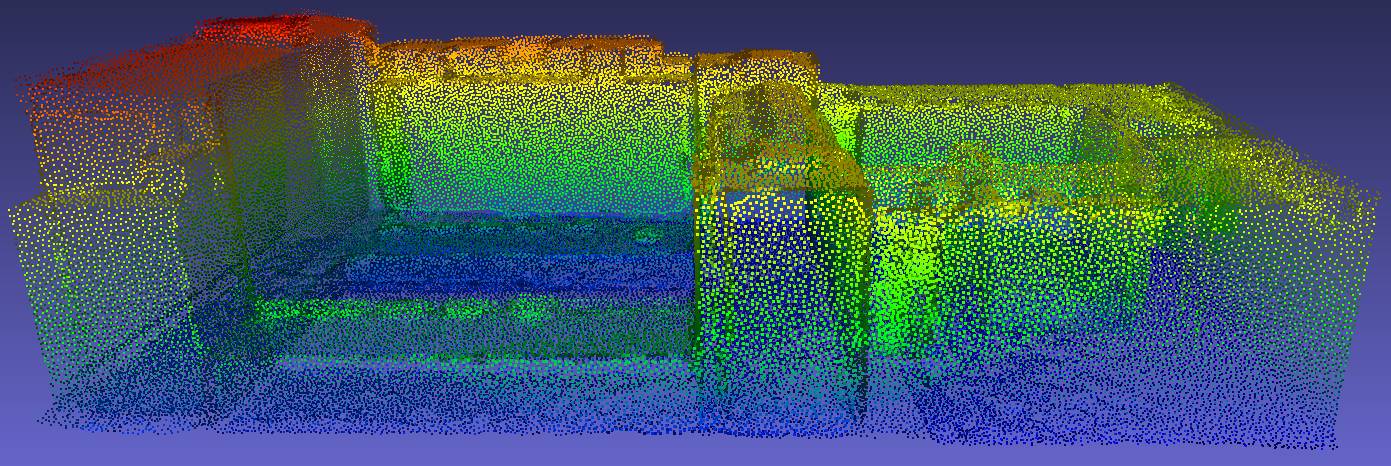
\includegraphics[height=1.5cm]{images/difference_mesh_model/pc_building_bercy}
                            \caption{3D point cloud of a building ($\approx 1.2\mathrm{e}{5}$ points).}
                        \end{center}
                    \end{subfigure}
                    \begin{subfigure}{.45\textwidth}
                        \begin{center}
                            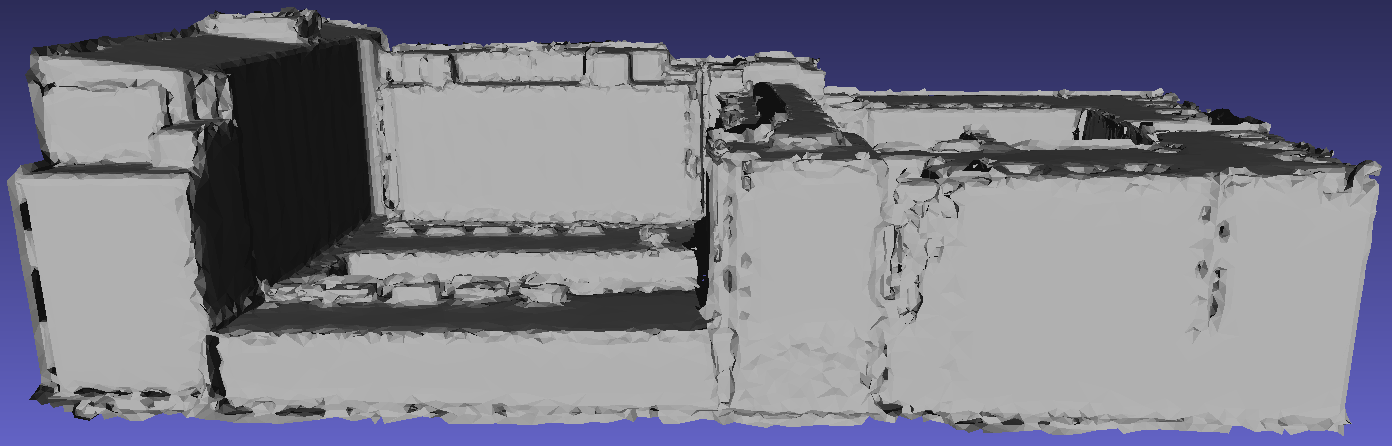
\includegraphics[height=1.5cm]{images/difference_mesh_model/bercy_building_mesh_1_e5}
                            \caption{3D mesh representing a building surface ($\approx 9.9\mathrm{e}{4}$ triangles).}
                        \end{center}
                    \end{subfigure}
                    \\
                    \begin{subfigure}{\textwidth}
                        \begin{center}
                            \includestandalone[mode=buildnew, height=3cm]{ground_truth_model}
                            \caption{Building 3D polyhedral model (1, 912 triangles).}
                        \end{center}
                    \end{subfigure}
                \end{center}
            \end{figure}
        \end{frame}
\end{document}